\chapter{Implémentation}

\section{Interface Web}

Nous avons utilisé la technologie JSF pour faire l'Interface Web. cela a été
grandement simplifié par l'utilisation du Plugin Visual JSF, qui permet de créer
une interface graphique et le code associé très facilement.

Pour l'image Google Map, elle a été créée à partir du service Static Maps API
V2.\\

\begin{figure}[!h]
	\centering
	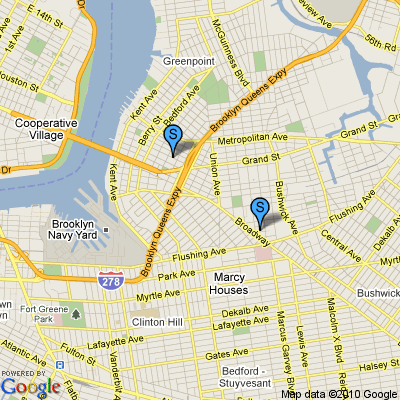
\includegraphics[scale=0.5]{staticmap.png}
	\caption{exemple d'image Google Map}
	\label{staticmap}
\end{figure}

Le principe est simple : il suffit de construire une url selon une méthodologie
particulière, et de la déclarer en tant qu'image url. Il est possible de
construire ainsi des url plutôt complexe permettant d'afficher des chemins
prédéfinis, les routes, \ldots

\clearpage

Par exemple, l'url permettant d'afficher l'exemple de l'image précédente :

\begin{verbatim}
http://maps.google.com/maps/api/staticmap?
center=Brooklyn+Bridge,New+York,NY
&zoom=14&size=512x512
&maptype=roadmap
&markers=color:blue|label:S|40.702147,-74.015794
&markers=color:green|label:G|40.711614,-74.012318
&markers=color:red|color:red|label:C|40.718217,-73.998284
&sensor=false
\end{verbatim}



\section{Web Services}

	\subsection{InterfaceManager}
	
		Ce service est un BPEL simple, qui effectue des requetes FIND dans les tables
		de type Information (figure\ref{bdd}) en fonction des champ remplie dans la
		requete.
	
	\subsection{ReservationManager}

		Ce service est une application composite de BPEL, qui comprend :
		\begin{itemize}
		  \item ReservationManager : BPEL central, il permet de coordonné tout les
		  autres BPEL et qui enregistre la reservation des reservations.
		  \item ClientManager : BPEL qui vérifie l'existance d'un client et qui
		  permet de récupérer son Id en partant de ses nom et prenom.
		  \item ReservManif : BPEL qui vérifie qu'une manifestation existe et qu'il y
		  a encors de la place. Et enregistre une reservation pour cette
		  manifestation.
		  \item ReservHotel : BPEL qui vérifie qu'un hotel existe et qu'il y a encors
		  de la place à une date donnée. Et enregistre une reservation pour cet
		  hotel.
		  \item ReservRestau : BPEL qui vérifie qu'un restaurant existe et qu'il y a
		  encors de la place à une date donnée. Et enregistre une reservation pour ce
		  restaurant.
		\end{itemize}
		
		les vérifications sont effectué grâce à toutes les tables, et les reservation
		sont enregistrées dans les tables de type Réservation (figure\ref{bdd}).
		
		Si une reservation est un succès ReservationManager renvoie 'OK' a l'Interface
		sinon un message d'erreur précisant le problème.

\section{BDD Manager}

\clearpage




















